\section{Experimental Setting}
\label{sec:real_world_exp_setting}
In this section, the experimental setup is explained and defined. Figure \ref{fig:workspace} illustrates the workspace where the robot operates, and compares it to the corresponding simulation environment. As can be observed, the simulation environment closely resembles the real-world counterpart. Both environments consist of the same robot agent, with identical camera configurations and workspace setup.

\begin{figure}[t]
    \centering
    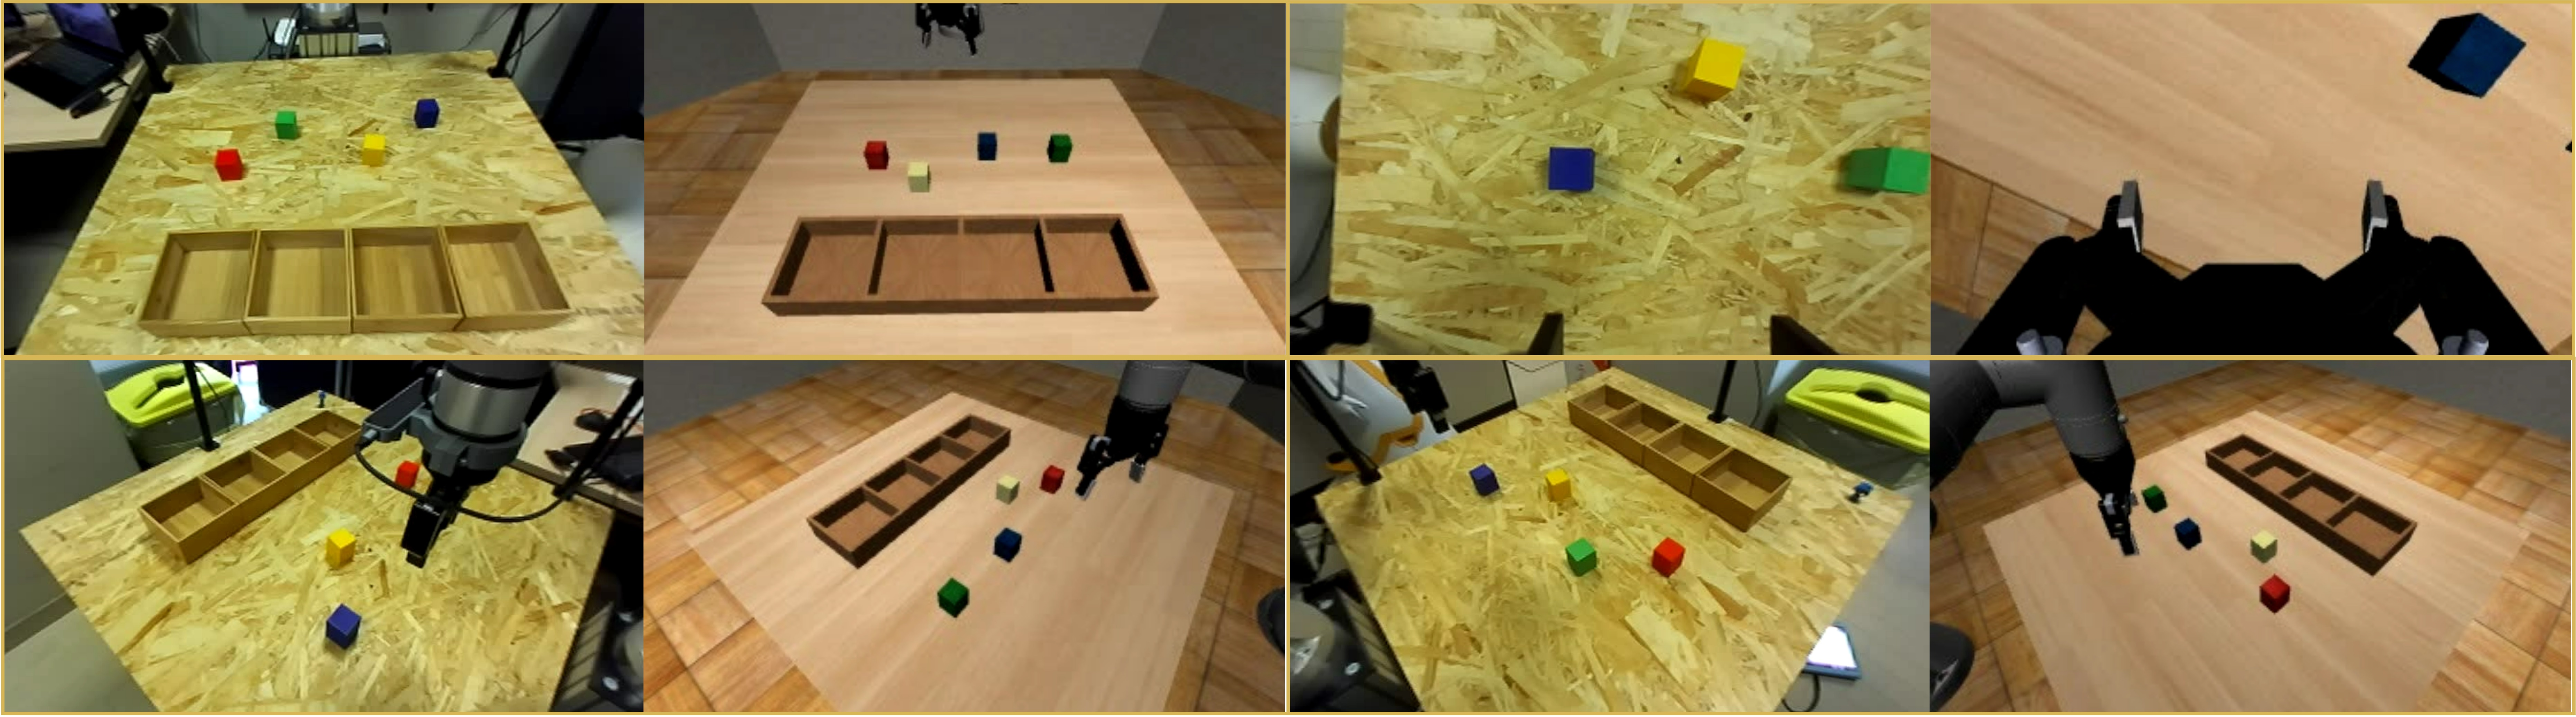
\includegraphics[width=1.0\textwidth]{figures/images/ch5/workspace.jpg}
    \caption{Workspace comparison between real-world (left) and simulated (right) scenarios. Images are taken from the frontal camera (Top-Left), the gripper camera (Top-Right), lateral-left camera (Bottom-Left) and lateral-right (Bottom-Right).}
    \label{fig:workspace}
\end{figure}

Specifically, the experimental setup includes:
\begin{itemize}
    \item The Universal Robots UR5e robot \cite{ur5e}, equipped with the Robotiq 2F-85 gripper \cite{robotiq}, which acts as the agent.
    \item Four Zed-Mini stereo cameras \cite{zed}, one camera is \\ mounted on the gripper, while the remaining three are positioned around the robot to ensure complete coverage of the workspace.
    \item A 100$\times$100 cm working table.
\end{itemize}

The reason for maintaining a high similarity between the real-world and simulation environments is to evaluate the potential for pre-training the model on a large and comprehensive simulation dataset, followed by fine-tuning on a smaller and incomplete real-world dataset. This approach allows leveraging the advantages of simulation for initial training while adapting the model to real-world conditions with minimal additional data.
